\documentclass[
  manuscript=article,  %% article (default), rescience, data, software, proceedings, poster
  layout=preprint,  %% preprint (for submission) or publish (for publisher only)
  year=20xx,
  volume=x,
]{extra/joas}

\doi{xx.xxxxx/joas.xxxx.xxxx}

\received {1 April 20xx}
\revised  {1 May 20xx}
\accepted {10 May 20xx}
\published{20 May 20xx}

\editor{Editor Name}

\reviewers{First Reviewer, Second Reviewer, Third Reviewer}

\addbibresource{reference.bib}

\DeclareRobustCommand{\equalcontribution}{\par\textsuperscript{\textdagger}These authors contributed equally to this work.}

\title{Recording-Aware Ensembles for Taxi-Out Time Estimation at Ten European Airports}

\author{Juan Esteban Lamilla Cuellar\texorpdfstring{\textsuperscript{\textdagger}}{}}
\affiliation{University of Alberta, Edmonton, Canada\equalcontribution}
\email{jlamilla@ualberta.ca}

\author{Michael Urbiztondo\texorpdfstring{\textsuperscript{\textdagger}}{}}
\affiliation{University of Alberta, Edmonton, Canada\equalcontribution}

\author{Abhinav Parbhakar\texorpdfstring{\textsuperscript{\textdagger}}{}}
\affiliation{University of Alberta, Edmonton, Canada\equalcontribution}

\author{Charles Ancheta\texorpdfstring{\textsuperscript{\textdagger}}{}}
\affiliation{University of Alberta, Edmonton, Canada\equalcontribution}

\keywords{taxi-out time; airport surface operations; label noise; ensemble learning; validation}

\abbreviations{
    ADS-B: Automatic Dependent Surveillance-Broadcast,
    EOBT: Estimated Off-Block Time,
    LOBT: Last known Off-Block Time in the flight plan,
    RMSE: Root Mean Square Error
}


\begin{document}

\begin{abstract}
Taxi-out time, the interval between an aircraft leaving its stand and taking off, drives fuel burn on the ground and enters the take-off times on which network planning relies. Many estimation studies treat the recorded off-block time as a physical event and validate on random splits of short, single-airport samples. For 2,085,047 departures at ten large European airports in 2025, we show that the recorded label has exploitable structure. Flight-plan records appear to have been attached to movements only when the recorded off-block stamp lay within 3,606 s of the last flight-plan off-block time, a tolerance we infer from the data, so every matched departure carries a provable interval for its label, and a missing flight plan is itself informative. Off-block stamps coincide with the scheduled time on 4.8\% of departures; at one airport (Rome Fiumicino) this happens on 18.1\% of departures against 2.5\% one minute either side, which indicates a recording artefact. Because the error measure is computed on the recorded label, we model it as a mixture of recording classes. The members are two-stage gradient-boosted trees, a distributional transformer whose histogram is masked to the feasible interval, and a class-structured combiner whose experts include an earlier stack of tabular, sequence and set models. A per-lane non-negative blend and label-free projections complete the estimator. Components are selected with month-held, nested cross-validation and, for ordinary changes, day-block bootstrap intervals under decision rules calibrated by null comparisons. On held-out months of 2025 the blend reaches an RMSE of 191.1 s (95\% interval 183.5 to 201.7 s) when 15 day-rollover records are excluded, and 227.4 s on all records. Error concentrates in departures without a flight plan and long delays. We also describe a label-free check for input drift and a consistency requirement for the inputs of stacked models.
\end{abstract}


% =====================================================================================
\section{Introduction}
\label{sec:introduction}

Taxi-out time is the time between an aircraft's off-block and its take-off. It matters for three reasons. First, it is the largest driver of the fuel burnt during taxi-out \cite{khadilkar2012estimation}: congestion can lengthen taxi-out to two or three times its unimpeded value at busy airports \cite{simaiakis2010impact}, and stop-and-go movement caused by congestion accounts for a sizeable share of taxi fuel \cite{nikoleris2011detailed}. Second, it links the off-block and take-off milestones on which collaborative decision making and the European network depend. In Airport Collaborative Decision Making the target take-off time is the target off-block time plus an estimated taxi-out time \cite{eurocontrol2017airport}, and the European performance scheme defines the Network Manager's estimated take-off time in the same way \cite{europeancommission2019commission}. Third, the additional taxi-out time, the actual time minus an unimpeded reference, is a monitored performance indicator in Europe and in the ICAO Global Air Navigation Plan \cite{europeancommission2019commission,icao2016description,eurocontrol2023additional}.

Taxi-out has been estimated with queueing models \cite{pujet1999inputoutput,idris2002queuing,simaiakis2016queuing}, regression and early machine learning \cite{jordan2010statistical,srivastava2011improving,ravizza2014aircraft,lee2016taxiout,lordan2016forecasting,diana2018can}, and, more recently, gradient-boosted trees, graph neural networks and other deep models \cite{wang2021aircraft,lim2021variable,swatowska2025generalisable,yin2024prediction}. Two gaps in this literature motivate the present work. The first concerns the label. Studies usually treat the recorded off-block time as the physical moment the aircraft left the stand \cite{swatowska2025generalisable,yuan2024additional}, and handle implausible records by trimming outliers \cite{wang2021aircraft,swatowska2025generalisable,yuan2024additional}. Yet the airport data specification used for European monitoring does not prescribe how the off-block time is captured and tolerates a share of implausible records \cite{eurocontrol2019specification}, and earlier work reports minute-rounded, missing and erroneous gate-out times \cite{pujet1999inputoutput,hotle2016using,lee2016taxiout}. When the error measure is computed on the recorded value, the quantity to predict is the conditional mean of that recorded value \cite{gneiting2011making}, artefacts included. The second concerns validation. Many recent studies evaluate on random splits, often of a few days or weeks at a single airport \cite{wu2026interpretable,tang2025road,tran2020taxispeed}; a recent three-airport study also uses a random split \cite{yang2026analysis}. Random splits leak within-day conditions such as weather, runway configuration and recording behaviour, and they tend to underestimate prediction error when observations are dependent \cite{roberts2017cross}.

This paper describes an estimator built for the recorded label and validated on held-out months. The data are 2,085,047 departures from ten large European airports in 2025, each with its movement record and, where available, its flight-plan fields. The contributions are:

\begin{enumerate}
  \item An analysis of the recorded label. Flight-plan records appear to have been attached only when the off-block stamp lay within 3,606 s of the flight plan's last off-block time, which gives every matched departure a provable label interval and makes a missing flight plan informative. Stamps that coincide with the schedule form a point mass whose excess over neighbouring minutes is concentrated at one airport.
  \item A modelling approach that treats the label as a mixture of recording classes with a computable point mass. We implement it in gradient-boosted trees, in a distributional transformer with a masked histogram head, and in a class-structured combiner over heterogeneous experts.
  \item A validation protocol for dependent operational data: month-held, nested cross-validation, day-block bootstrap intervals, and decision rules fixed in advance and calibrated with null comparisons.
  \item Practical findings on the deployment of stacked estimators: a label-free way to estimate the effect of drift in a single input, and the requirement that a stacked model's inputs be generated in the same way at training and prediction time.
\end{enumerate}

Section~\ref{sec:related} reviews related work. Section~\ref{sec:data} describes the data and the structure of the label. Section~\ref{sec:method} presents the estimator and Section~\ref{sec:validation} the validation protocol. Section~\ref{sec:results} reports results and Section~\ref{sec:discussion} discusses them.


% =====================================================================================
\section{Related work}
\label{sec:related}

\subsection{Estimating taxi-out time}

Early work at the Massachusetts Institute of Technology modelled taxi-out as unimpeded travel plus runway queueing. Pujet et al.\ built a stochastic input-output model of the Boston departure process \cite{pujet1999inputoutput}. Idris et al.\ found that the number of departures scheduled to take off ahead of a flight was the single most important factor, and their queue model reduced mean absolute error by about 20\% relative to a 14-day running average \cite{idris2002queuing}. Arrivals also lengthen taxi-out \cite{clewlow2010impact}. The queueing model of Simaiakis and Balakrishnan predicts the expected taxi-out and its variance for each flight, given the pushback schedule \cite{simaiakis2016queuing}. Off-block times themselves are uncertain: estimated off-block times can be several minutes wrong, with errors that grow with look-ahead time and are skewed \cite{badrinath2020impact}, and an analysis of pushback forecasts at Frankfurt argued that their errors could not be reduced by more than a factor of two or three \cite{carr2004robust}.

Statistical and machine-learning studies followed: reinforcement learning \cite{balakrishna2008airport}, regression on surface-surveillance data, with subset selection in one case \cite{jordan2010statistical,srivastava2011improving}, fuzzy rule-based systems and support vector regression at Zurich and Stockholm \cite{ravizza2013combined,ravizza2014aircraft}, comparisons of standard learners at Charlotte \cite{lee2016taxiout}, Seattle \cite{diana2018can} and Paris-Charles de Gaulle \cite{herrema2018taxiout}, and a regression model at Barcelona \cite{lordan2016forecasting}. Wang et al.\ compared learners at Manchester, Zurich and Hong Kong using ADS-B tracks from a commercial provider, found random forests best, with queue length and taxi distance among the most important features \cite{wang2021aircraft}. A graph transformer at Atlanta improved on gradient boosting with the same features by about 3\% in RMSE \cite{lim2021variable}. A recent study pooled six European airports in one CatBoost model and tested on a later year \cite{swatowska2025generalisable}. A 2024 review names low data quality and the lack of distributional prediction as open problems \cite{yin2024prediction}. Distributional outputs are still rare; examples include discrete conditional taxi-time distributions \cite{liu2026stochastic} and, for related quantities, mixture-density delay predictions \cite{zoutendijk2021probabilistic} and quantile forecasts of departure flow \cite{zhou2025riskaware}.

Across these studies the target differs (pushback to take-off, gate-out to wheels-off, spot to runway queue, pushback to line-up), so reported accuracies are not directly comparable. Recorded labels are known to be imperfect \cite{pujet1999inputoutput,hotle2016using,lee2016taxiout,lordan2016forecasting}, but among the works we reviewed none models how the off-block stamp was recorded.

\subsection{Point-mass mixtures and label noise}

Under squared error the optimal point prediction is the conditional mean of the quantity being scored \cite{gneiting2011making,savage1971elicitation}. When that quantity mixes a point mass with a continuous part, its mean decomposes by total expectation into class probabilities and class-conditional means \cite{belotti2015twopm}. Two-part, hurdle and zero-inflated models use this structure \cite{duan1983comparison,mullahy1986specification,lambert1992zero}, and mixtures of experts implement it with an input-dependent gate \cite{jacobs1991adaptive,jordan1994hierarchical}. Label noise whose probability depends on the inputs is not noise at random \cite{frenay2014classification}. Unlike classical mean-zero error in a response, misclassification-type errors bias what a model learns \cite{hausman2001mismeasured}. If the scored label carries the same corruption at test time, it should be modelled rather than cleaned. Distributional heads trained by classification over histogram bins \cite{imani2018improving,farebrother2024stop} and binned output distributions in tabular transformers \cite{muller2022transformers,hollmann2025accurate} provide a convenient way to represent such mixtures.

\subsection{Tabular models, ensembles and validation}

Gradient-boosted trees \cite{friedman2001greedy,chen2016xgboost,prokhorenkova2018catboost,ke2017lightgbm} remain strong on tabular data of moderate size \cite{grinsztajn2022why,mcelfresh2023when}. Deep tabular models can match them on some benchmarks \cite{gorishniy2021revisiting,holzmuller2024better,gorishniy2025tabm}, and ensembles across model families tend to beat single families \cite{shwartzziv2022tabular,erickson2025tabarena}. Stacking fits combination weights on cross-validated predictions \cite{wolpert1992stacked,breiman1996stacked,vanderlaan2007super}. In forecast combination, estimated weights often lose to equal weights because the weights are estimated with error \cite{smith2009simple,claeskens2016forecast}. Under temporal or grouped dependence, blocked cross-validation is preferred to random splits \cite{roberts2017cross,arlot2010survey}, since standard $K$-fold cross-validation requires uncorrelated errors \cite{bergmeir2018note}, tuning must be nested inside the validation loop \cite{varma2006bias,cawley2010overfitting}, and resampling for uncertainty must respect clusters \cite{field2007bootstrapping,cameron2008bootstrapbased}.


% =====================================================================================
\section{Data and the structure of the label}
\label{sec:data}

\subsection{Data}

The data cover the movements at ten European airports in 2025, as released by the data provider, which removed military, head-of-state and sensitive flights: Frankfurt (EDDF), Munich (EDDM), London Heathrow (EGLL), Amsterdam Schiphol (EHAM), Barcelona (LEBL), Madrid (LEMD), Paris-Charles de Gaulle (LFPG), Rome Fiumicino (LIRF), Zurich (LSZH) and Istanbul (LTFM). There are 4,167,797 movements, of which 2,085,047 are departures (Table~\ref{tb:airports}). Each movement record gives the take-off (or landing) time, the recorded off-block (or in-block) time, the scheduled time, stand, runway and aircraft type. Where the data provider could match the movement to a Network Manager flight, the record also carries flight-plan fields, among them the estimated off-block time of the filed flight plan (EOBT), the last known off-block time (LOBT), the initial off-block time and an off-block time derived from the flown trajectory. 22,470 departures (1.08\%) have no flight-plan record; on these rows every flight-plan field is empty.

The label is the recorded taxi-out time
\begin{equation}
y = t_{\mathrm{TO}} - t_{\mathrm{OB}},
\label{eq:label}
\end{equation}
where $t_{\mathrm{TO}}$ is the recorded take-off time and $t_{\mathrm{OB}}$ the recorded off-block time, in seconds. This matches the official definition of taxi-out time as the actual take-off time minus the actual off-block time \cite{eurocontrol2023additional,eurocontrol2017airport}. Its median is 912 s and its mean 991 s. 369 labels are negative (minimum $-12$ s) and 4,126 exceed one hour.

The setting is post-operational. For every departure to be estimated, the take-off time, the schedule, the flight-plan fields and all other movements at the airport, including arrivals with their in-block times, are known; only the departure's own off-block stamp is not. The estimator therefore reconstructs a recorded duration after the fact, and its accuracy is not comparable with that of tactical predictors that run before off-block.

\begin{table}[htbp!]
  \centering
  \small
  \caption{Departures in 2025 by airport. Flight plan: share of departures with a Network Manager flight-plan record. Schedule-coincident: share whose off-block stamp lies within 10~s of the scheduled time. Delay $\geq$ 1~h: share with take-off at least one hour after the scheduled off-block time.}
  \label{tb:airports}
  \begin{tabular}{lrrrrr}
  \toprule
  \textbf{Airport} & \textbf{Departures} & \textbf{Flight plan} & \textbf{Schedule-} & \textbf{Median} & \textbf{Delay} \\
  & & \textbf{(\%)} & \textbf{coincident (\%)} & \textbf{label (s)} & \textbf{$\geq$ 1 h (\%)} \\
  \midrule
  EDDF & 230,141 & 99.2 & 1.2 & 837 & 8.5 \\
  EDDM & 167,334 & 99.4 & 5.0 & 774 & 5.9 \\
  EGLL & 239,546 & 99.4 & 4.9 & 1,319 & 9.8 \\
  EHAM & 247,951 & 98.4 & 1.3 & 742 & 9.9 \\
  LEBL & 179,705 & 99.0 & 5.6 & 906 & 10.7 \\
  LEMD & 212,242 & 99.6 & 4.5 & 985 & 9.7 \\
  LFPG & 239,552 & 98.4 & 4.1 & 954 & 12.5 \\
  LIRF & 160,704 & 99.1 & 18.1 & 1,025 & 10.8 \\
  LSZH & 134,907 & 98.3 & 1.1 & 711 & 7.3 \\
  LTFM & 272,965 & 98.7 & 5.1 & 963 & 7.7 \\
  \midrule
  All & 2,085,047 & 98.9 & 4.8 & 912 & 9.4 \\
  \bottomrule
  \end{tabular}
\end{table}

External inputs are all openly available. Ground tracks within 12 km of each airport come from the ADSB.lol global history archive \cite{adsblol2026historical}, a crowdsourced ADS-B collection whose coverage depends on receivers in line of sight, as for other crowdsourced networks \cite{schafer2014bringing,strohmeier2021crowdsourced}; runway thresholds come from OurAirports \cite{ourairports2026open}; taxiway geometry from OpenStreetMap \cite{haklay2008openstreetmap}; stand attributes from the X-Plane Scenery Gateway \cite{xplane2026scenery}; weather from METAR reports in the Iowa Environmental Mesonet archive \cite{iem2026download} and the Open-Meteo historical service \cite{zippenfenig2023openmeteo}; and daily airport arrival air traffic flow management delay from EUROCONTROL \cite{eurocontrol2026airport}. The estimator was also applied to departures in January, February, June and July 2026, for which only inputs were available; we use these months only for label-free diagnostics: input drift (Section~\ref{sec:drift}) and the consistency of stacked inputs (Section~\ref{sec:consistency}).

\subsection{The flight-plan matching window}
\label{sec:window}

On every one of the 2,062,577 departures with a flight-plan record, the recorded off-block stamp lies within 3,606 s of the LOBT, and the maximum is exactly 3,606 s (Figure~\ref{fig:anatomy}b). The distribution is cut sharply at that value, so we read it as the tolerance of the matching step. We observed this tolerance in the data and found no documentation of it. Two consequences follow. With $m = t_{\mathrm{TO}} - t_{\mathrm{LOBT}}$, every matched departure satisfies
\begin{equation}
m - 3606 \;\leq\; y \;\leq\; m + 3606,
\label{eq:window}
\end{equation}
a label interval that is known before the label is seen. And a departure without a flight-plan record is partly a departure whose stamp fell outside the window, so its label distribution differs from that of matched departures. The matching is a deterministic record-linkage rule \cite{fellegi1969theory}, and the resulting missingness depends on the label \cite{rubin1976inference,heckman1979sample}. A model fitted only to matched departures, or one that imputes the missing flight-plan fields, ignores this information.

\begin{figure}[htbp!]
  \centering
  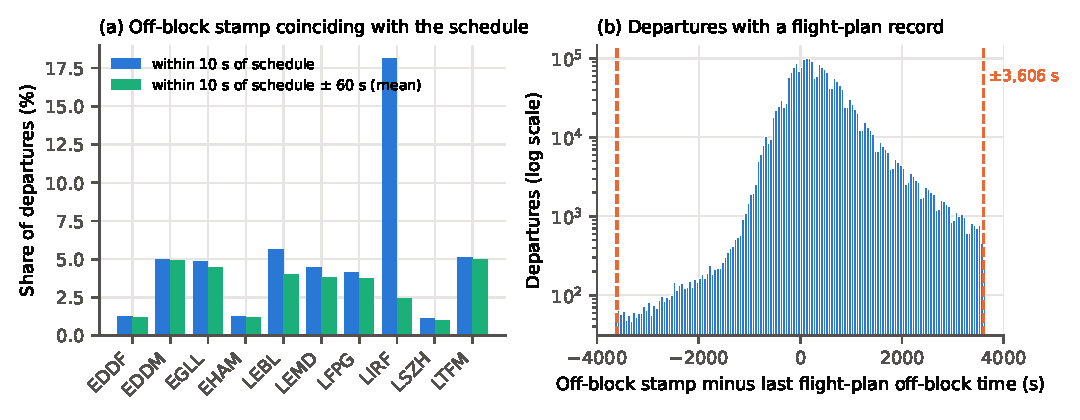
\includegraphics[width=\textwidth]{figures/label_anatomy.pdf}
  \caption{Structure of the recorded label, 2025 departures. (a) Share of departures whose off-block stamp lies within 10~s of the scheduled time, against the mean share within 10~s of the scheduled time plus or minus 60~s. Outside LIRF the two are much closer, as expected when stamps and schedules are recorded to the minute; at LIRF the coincidence is seven times its neighbours. (b) Off-block stamp minus the last flight-plan off-block time for departures with a flight-plan record; no value exceeds 3,606~s in magnitude.}
  \label{fig:anatomy}
\end{figure}

\subsection{Recording classes}
\label{sec:classes}

The recorded stamp is not always a physical event. We distinguish the following recording classes, defined on training rows from the stamp and therefore never used as inputs.

\textit{Schedule-coincident stamps.} On 100,049 departures (4.80\%; 100,048 once the one rollover among them is excluded) the stamp lies within 10 s of the scheduled off-block time. The label is then $y \approx C$, with $C = t_{\mathrm{TO}} - t_{\mathrm{SCHED}}$, a quantity known for every departure. Part of this mass reflects minute-resolution recording: outside LIRF, the share within 10 s of the schedule is close to the share within 10 s of the schedule plus or minus one minute (Figure~\ref{fig:anatomy}a). At LIRF it is 18.1\% against 2.5\%, consistent with a recording practice in which the scheduled time stands in for the off-block time. Summed over airports, the excess over neighbouring minutes is about 32,300 departures (1.6\%), of which about 25,100 are at LIRF. For prediction the cause does not matter: whenever the stamp equals the schedule the label equals $C$, so the probability of that event is worth estimating. On 3.2\% of matched departures the schedule lies more than 3,616 s from the LOBT; there, Equation~\eqref{eq:window} rules the coincidence out, and its probability is set to zero.

\textit{Near-schedule stamps.} 139,055 departures (6.7\%) have a stamp between 10 s and 15 min from the schedule while taking off more than 30 min after it. These tend to carry long labels (median 1,497 s). We model them as $C$ minus a learnt offset.

\textit{Long stamps.} 1,250 departures outside the classes above have labels above one hour. They include 31 departures with a flight plan and $C < 1$~h, whose stamp lies 16 to 115 min ahead of the schedule. Another 84 matched departures with $C < 1$~h and a label above one hour fall in the near-schedule class; Table~\ref{tb:errorshare} counts all 115 together.

\textit{Day rollovers.} Fifteen departures (13 at LIRF) have labels near 86,400 s: the stamp carries the previous day's date. Fourteen of them have no flight-plan record; on the one that does, the LOBT carries the same earlier date and the label equals $m$ to within 1 s. They are excluded from training and reported separately.

The airport data specification tolerates such records: it requires the taxi-out time to be positive and below 60 min for at least 95\% of flights and does not prescribe how the off-block time is captured \cite{eurocontrol2019specification}. The official indicator excludes taxi-out times above 120 min and flights de-iced after off-block \cite{eurocontrol2023additional}; the label studied here keeps them.

\subsection{Decomposition of the squared error}
\label{sec:errorshare}

Squared error concentrates in a few groups of rows. Table~\ref{tb:errorshare} decomposes the squared error of the blend's month-held predictions after window projection (Section~\ref{sec:results}). Fifteen rollover rows hold 29\% of it. Departures without a flight plan (1.1\% of rows) and matched departures delayed by at least one hour (8.6\%) hold another 32\%. The remaining 90\% of departures hold 39\%. Any comparison pooled over all rows is therefore dominated by a handful of records. We report the overall result both on all rows and with rollovers excluded, every breakdown with rollovers excluded, and we organise the blend into four lanes: matched departures with $C<1$~h, matched departures with $C \geq 1$~h, unmatched departures at LIRF, and unmatched departures elsewhere.

\begin{table}[htbp!]
  \centering
  \small
  \caption{Decomposition of the squared error of the blend's month-held predictions for 2025, after window projection. $C$: take-off time minus scheduled off-block time.}
  \label{tb:errorshare}
  \begin{tabular}{lrrrr}
  \toprule
  \textbf{Rows} & \textbf{Count} & \textbf{Rows} & \textbf{Squared} & \textbf{RMSE} \\
  & & \textbf{(\%)} & \textbf{error (\%)} & \textbf{(s)} \\
  \midrule
  Day rollovers & 15 & $<$0.01 & 29.4 & 45,956 \\
  No flight plan (rollovers excluded) & 22,456 & 1.08 & 15.6 & 864 \\
  Flight plan, $C \geq 1$ h & 179,947 & 8.63 & 16.1 & 311 \\
  Flight plan, $C < 1$ h, label $>$ 1 h & 115 & 0.01 & 0.4 & 1,823 \\
  Everything else & 1,882,514 & 90.29 & 38.6 & 149 \\
  \bottomrule
  \end{tabular}
\end{table}


% =====================================================================================
\section{Method}
\label{sec:method}

Figure~\ref{fig:overview} summarises the estimator. A feature matrix with one row per departure feeds a set of members. Each member predicts the recorded label as a mixture of recording classes. A class-structured combiner merges the members' class-level outputs, a per-lane blend combines the strongest members, and label-free post-processing completes the estimate. Appendix~\ref{app:settings} lists the settings of the main members.

\begin{figure}[htbp!]
  \centering
  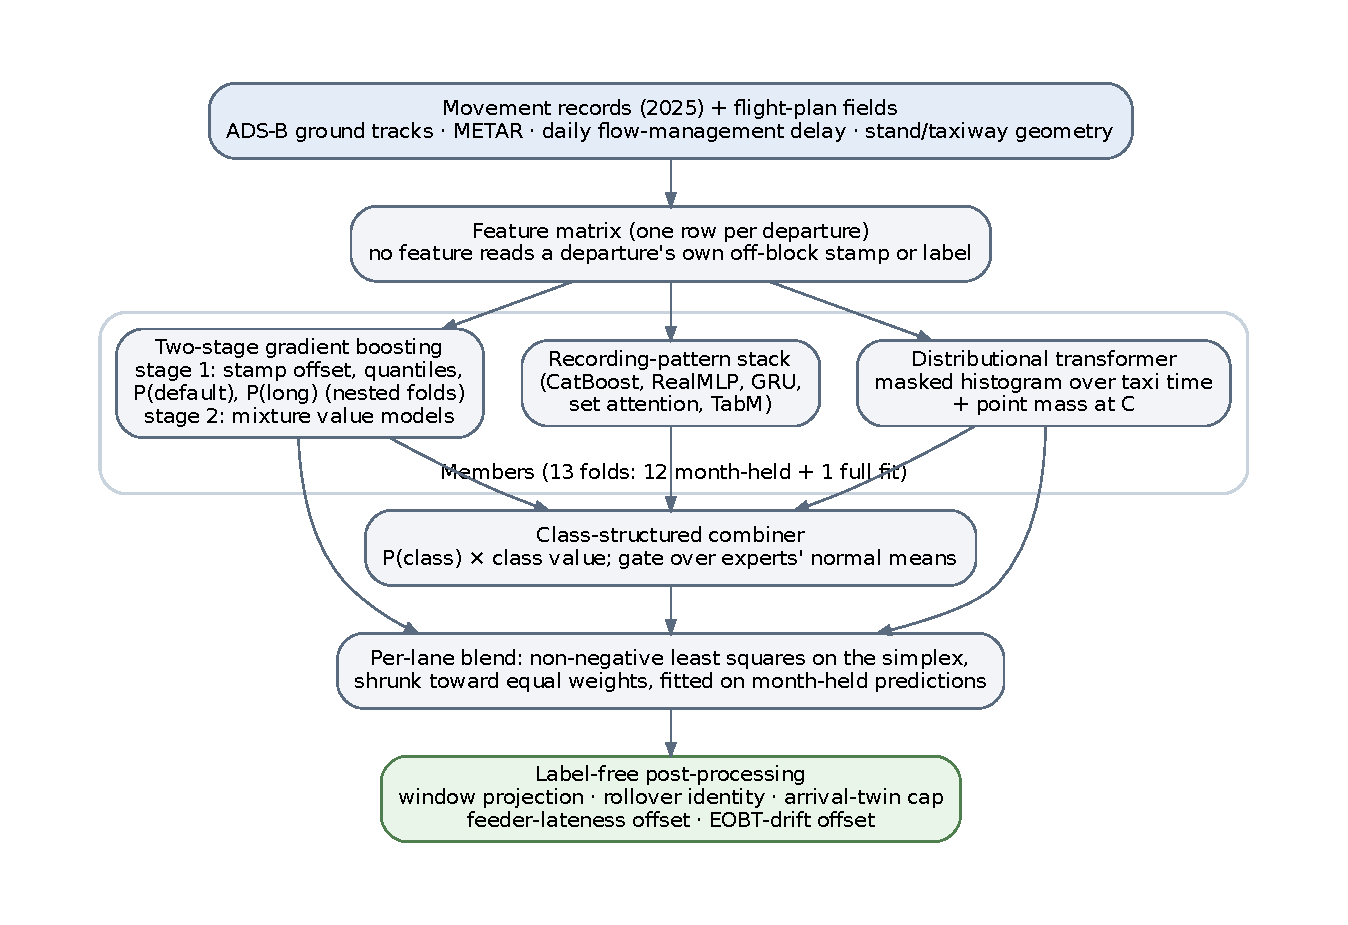
\includegraphics[width=0.85\textwidth]{figures/method_overview.pdf}
  \caption{Overview of the estimator. Every member is trained 13 times: once for each held-out month of 2025 and once on the full year.}
  \label{fig:overview}
\end{figure}

\subsection{Target and mixture formulation}
\label{sec:mixture}

Because the error measure is the RMSE of the recorded label, the target is $\mathbb{E}[y \mid \mathbf{x}]$ \cite{gneiting2011making}. With recording classes $k$, class probabilities $p_k(\mathbf{x})$ and class-conditional means $v_k(\mathbf{x})$, total expectation gives
\begin{equation}
\mathbb{E}[y \mid \mathbf{x}] = \sum_k p_k(\mathbf{x})\, v_k(\mathbf{x}),
\label{eq:mixture}
\end{equation}
the same decomposition that underlies two-part and zero-inflated models \cite{belotti2015twopm,lambert1992zero}. For schedule-coincident stamps $v_k = C$ to within 10 s, so only the probability has to be learnt. The point mass is a recording outcome, so a censored-data model of a physical duration does not describe it \cite{belotti2015twopm,tobin1958estimation}. The simplest form used throughout is
\begin{equation}
\hat{y} = \hat{p}_{\mathrm{def}}\, C + (1-\hat{p}_{\mathrm{def}})\, \hat{y}_{\mathrm{normal}},
\label{eq:twopart}
\end{equation}
with $\hat{p}_{\mathrm{def}}$ set to zero where the window of Equation~\eqref{eq:window} excludes the coincidence.

\subsection{Features}
\label{sec:features}

No feature reads the off-block stamp or the label of the departure it describes. Departure labels enter features only through nested stage-1 predictions and fold-scoped target encodings. Because the setting is post-operational, features may use other movements' take-off and in-block times on both sides of the departure. Table~\ref{tb:features} lists the feature families; the gradient-boosted, transformer and combiner members use a compact matrix, and some families exist only in the recording-pattern stack (Section~\ref{sec:stack}). Several follow the literature: queue length and the number of movements during taxi-out \cite{idris2002queuing,clewlow2010impact,wang2021aircraft}, stand, runway and taxi distance \cite{jordan2010statistical,lordan2016forecasting,kato2022applying}, weather and de-icing \cite{eurocontrol2011algorithm,schultz2018weather}, air traffic flow management regulation \cite{yuan2024additional}, and the lateness of the inbound aircraft as a reactionary-delay mechanism \cite{ahmadbeygi2008analysis,kafle2016modeling,eurocontrol2025allcauses}. Taxi distances are shortest paths on the OpenStreetMap taxiway graph, computed with Dijkstra's algorithm \cite{dijkstra1959note} as implemented in SciPy \cite{virtanen2020scipy}. Target encodings by airport crossed with runway, stand, operator and aircraft type are fitted inside each fold with shrinkage toward the global mean, following regularised target encoding \cite{miccibarreca2001preprocessing,pargent2022regularized}.

\begin{table}[htbp!]
  \centering
  \small
  \caption{Feature families. Families marked (S) are used only by the recording-pattern stack (Section~\ref{sec:stack}); the other members use a compact matrix of the remaining families. ``Window'' quantities use the take-off time $t_{\mathrm{TO}}$, which is known for every departure in this post-operational setting.}
  \label{tb:features}
  \begin{tabular}{p{0.27\textwidth}p{0.66\textwidth}}
  \toprule
  \textbf{Family} & \textbf{Content} \\
  \midrule
  Calendar and identity & hour, weekday, month; airport, runway, stand, operator, aircraft type, destination as categories \\
  Flight-plan times & take-off minus each flight-plan time (EOBT, LOBT, initial off-block time, trajectory-derived off-block time), their differences, schedule minus LOBT, the window bounds of Equation~\eqref{eq:window}, flags for a missing flight plan and an infeasible schedule coincidence \\
  Traffic and queues (S) & take-offs and landings in rolling windows, departures queued ahead, aircraft on the surface, gaps between runway movements, scheduled demand \\
  Neighbour taxi & median take-off minus trajectory-derived off-block time of matched departures within one hour, and their count \\
  Plan residuals & filed block-to-block time minus its median for the route (and route and aircraft type) \\
  Stand handover & time since the stand's previous arrival and departure; lateness of the arrival that fed the stand; stand attributes and taxiway-graph distance (S) \\
  Recording behaviour & schedule-coincidence shares of arrivals by operator, operator and month, operator and day, and airport and day; daily share of departures without a flight plan \\
  ADS-B ground track & time from first ground movement to take-off, path length, stop and hold times, mean ground speed, pushback signature, distance of the first point from the stand, coverage flag \\
  Weather (S) & visibility, ceiling, low-visibility procedures, frozen precipitation, de-icing likelihood (METAR, Open-Meteo); solar elevation and night-curfew distance \\
  Flow management & daily airport arrival air traffic flow management delay per flight, by cause; share of flights delayed more than 15 min \\
  Disruption calendar & flags from a hand-compiled calendar of strikes and disruptions (one member only) \\
  Target encodings (S) & airport crossed with runway, stand, stand and runway, operator, aircraft type: fold-scoped mean and quantiles with shrinkage \\
  \bottomrule
  \end{tabular}
\end{table}

\subsection{Two-stage gradient-boosted trees}
\label{sec:gbm}

The first family predicts properties of the off-block stamp before predicting the label. Stage~1 uses XGBoost \cite{chen2016xgboost} to estimate the offset $d = t_{\mathrm{OB}} - t_{\mathrm{LOBT}}$ with squared error, its 10th, 50th and 90th percentiles with the quantile loss \cite{koenker1978regression}, and the probabilities of a schedule-coincident stamp and of a label above one hour on a stamp that is not schedule-coincident, with the logistic loss. Because $y = m - d$ on matched departures, stage~1 turns the window of Equation~\eqref{eq:window} into an estimate and an interval. To keep stage-2 training rows free of in-fold stage-1 fits, the stage-1 features of each training row come from inner folds that hold out each of the eleven training months in turn \cite{varma2006bias,chernozhukov2018double}. Stage~2 fits the label with and without the stage-1 outputs, and fits a normal-class model on rows that are not schedule-coincident, which Equation~\eqref{eq:twopart} combines with $\hat{p}_{\mathrm{def}}$.

Three CatBoost variants \cite{prokhorenkova2018catboost} reuse the stage-1 outputs. The first fits the two-part mixture with a deep regressor. The second fits it separately for each airport. The third is a four-class stamp model: a multiclass classifier over normal, schedule-coincident, near-schedule and long stamps, with one value model per class. The normal class uses a regressor on the offset bounded by the window. The near-schedule class predicts $C$ minus a learnt offset. The long class uses a regressor on $\log(y-3600+1)$, retransformed with the normal-theory factor $\exp(s^2/2)$ \cite{belotti2015twopm}. The prediction is the probability-weighted mean of Equation~\eqref{eq:mixture}. The four-class model also receives, as features, the deviations of the recording-pattern stack's members from the stack's prediction (Section~\ref{sec:stack}). A homoskedastic retransformation is not consistent under heteroskedasticity \cite{belotti2015twopm,manning1998logged}, and $s^2$ is estimated on training residuals, so the factor is an approximation.

\subsection{Distributional transformer}
\label{sec:transformer}

The second family is an FT-Transformer \cite{gorishniy2021revisiting}. Each numeric feature becomes a token through a learnt affine map, with a learnt token for missing values; inputs are clipped to the 1st and 99th training percentiles and standardised. Each categorical feature becomes an embedding \cite{guo2016entity}. A class token passes through three pre-norm Transformer layers \cite{vaswani2017attention,xiong2020layer} of width 64 with four attention heads and dropout 0.1 \cite{srivastava2014dropout}. We use GELU activations \cite{hendrycks2016gaussian} where the original FT-Transformer uses ReGLU.

The head outputs $K+1$ logits: $K$ bins over the label (20 s wide up to one hour, 120 s wide up to four hours) and one atom at $y = C$. On matched departures, bins outside the window of Equation~\eqref{eq:window}, widened by 14 s, receive a logit of $-10^9$; the atom is masked where the coincidence is infeasible. Masking invalid outputs in a softmax is common practice \cite{huang2022closer}. The training target is the atom for schedule-coincident rows and, otherwise, a Gaussian-smoothed histogram (HL-Gauss) whose standard deviation is 0.75 bin widths (15 s and 90 s) \cite{imani2018improving,farebrother2024stop}. The loss is cross-entropy plus a small squared-error term on the distribution mean. The prediction is the mean of the predicted distribution, the RMSE-optimal summary (Section~\ref{sec:mixture}). Training uses AdamW \cite{loshchilov2019decoupled} with a one-cycle schedule \cite{smith2019superconvergence}, batches of 1,024, six epochs and bfloat16 arithmetic \cite{kalamkar2019study}. Predictions are averaged over seeds \cite{lakshminarayanan2017simple}. Variants differ in their inputs: the base model; a model that also receives the stage-1 outputs as tokens; a model with disruption-calendar tokens; an EOBT-free model without any feature anchored on the filed EOBT; and a model that upweights departures without a flight plan tenfold.

\subsection{Recording-pattern stack}
\label{sec:stack}

The third family is an earlier stack of seven members (Table~\ref{tb:stack}) built on a broader feature set (Table~\ref{tb:features}). Every member predicts on a square-root target and carries the same recording head: for each recording pattern $k$ whose value $C_k$ is computable at prediction time, an XGBoost classifier nested in the training fold estimates $p_k$, and the prediction is $\sum_k p_k C_k + (1-\sum_k p_k)\,\hat{y}_{\mathrm{normal}}$. Members trained with ADS-B features are paired with twins trained without them, and rows without a ground track are routed to the twin. On departures without a flight plan, a LightGBM \cite{ke2017lightgbm} lane model of the form of Equation~\eqref{eq:twopart} replaces the member where an inner month-held comparison favours it. A six-class neural mixture then models the label of every departure, with classes masked when observable facts rule them out. A cell-wise stacker combines the members with non-negative weights per airport, flight-plan status and delay band, shrunk toward parent cells; the shrinkage strength is chosen by inner month-held validation. Rows with $C \geq 1$~h are taken from an earlier version of the stack with unrouted members, which scored better on those rows in month-held validation (398.0 s against 400.3 to 400.8 s, without an interval); the earlier version was also kept because changes affecting these rows could not be validated for inputs without a 2025 counterpart. The stack's month-held prediction is one of the experts of the combiner (Section~\ref{sec:combiner}).

\begin{table}[htbp!]
  \centering
  \small
  \caption{Members of the recording-pattern stack. ``Routed'' members use an ADS-B-free twin on rows without a ground track. Weights are the global non-negative stacker weights; members with zero global weight still carry weight in some cells.}
  \label{tb:stack}
  \begin{tabular}{p{0.24\textwidth}p{0.5\textwidth}r}
  \toprule
  \textbf{Member} & \textbf{Description} & \textbf{Weight} \\
  \midrule
  GRU sequence model (routed) & bidirectional GRU \cite{cho2014learning,schuster1997bidirectional} over the airport's movement sequence around the departure, attention pooling; tuned with TPE & 0.445 \\
  RealMLP (routed) & RealMLP \cite{holzmuller2024better}; hyper-parameters from a TPE search & 0.309 \\
  Set attention (routed) & multi-head attention \cite{vaswani2017attention,lee2019set} over nearby movements & 0.148 \\
  CatBoost (routed) & depth 10, learning rate 0.02, taxi-distance and stand features; tail-prone features masked on rows without a flight plan & 0.098 \\
  CatBoost with GRU input & CatBoost receiving the out-of-fold GRU prediction & 0.000 \\
  RealMLP with taxi distance & RealMLP plus taxiway-graph distance & 0.000 \\
  TabM & parameter-efficient MLP ensemble \cite{gorishniy2025tabm,wen2020batchensemble} & 0.000 \\
  \bottomrule
  \end{tabular}
\end{table}

Hyper-parameters of the GRU and RealMLP members come from a tree-structured Parzen estimator search \cite{bergstra2011algorithms} in Optuna \cite{akiba2019optuna}, run on January and July with one seed and confirmed with three new seeds on the ten months the search never saw. A search for the set-attention member did not pass this confirmation.

\subsection{Class-structured combiner}
\label{sec:combiner}

The strongest single model is a class-structured combiner. For each departure it predicts
\begin{equation}
\begin{split}
\hat{y} = {}& P_{\mathrm{def}}\, C + P_{\mathrm{near}}\,\bigl(C - 300\,\mathrm{softplus}(a+1)\bigr) + P_{\mathrm{long}}\, v_{\mathrm{long}}\, e^{0.3\tanh b} \\
& + P_{\mathrm{normal}} \sum_j g_j\, n_j + 100\tanh(r/10),
\end{split}
\label{eq:combiner}
\end{equation}
where $(P_{\mathrm{def}}, P_{\mathrm{near}}, P_{\mathrm{long}}, P_{\mathrm{normal}})$ are class probabilities (with $P_{\mathrm{def}}$ masked where infeasible), $v_{\mathrm{long}}$ is the four-class model's long-class value, $n_j$ are the experts' predictions of the normal-class mean, each clipped to the window, $g_j$ are softmax gate weights, and $a$, $b$, $r$ are bounded adjustments. The experts are the gradient-boosted normal-class models, the transformers' conditional normal means $(\hat{y}_{\mathrm{FT}} - \hat{p}\,C)/(1-\hat{p})$, the stage-1 estimate $m - \hat{d}$, the recording-pattern stack, and several auxiliary models. One multilayer perceptron produces all outputs from an airport embedding and a context vector: $C$, $m$, the window, the hour, the coverage and feasibility flags, every member's class probabilities and quantiles, and each expert's deviation from the experts' mean, divided by 300 s. It has two hidden layers of 256 units with SiLU activations \cite{elfwing2018sigmoid} and zero-initialised gate and adjustment heads, so training starts from an equal-weight average \cite{bachlechner2021rezero}. The loss is the squared error of Equation~\eqref{eq:combiner} plus 0.1 times the cross-entropy of the observed class. This is a mixture of experts with an input-dependent gate \cite{jacobs1991adaptive,jordan1994hierarchical}, applied to pre-trained experts and therefore closer to stacking with class probabilities as level-one inputs \cite{ting1999issues}. One instance is trained on all departures (17 seeds); a second only on departures without a flight plan (45 seeds).

\subsection{Per-lane blend}
\label{sec:blend}

The members are combined separately in each of the four lanes of Section~\ref{sec:errorshare}. For lane data $\mathbf{X}$ (member predictions) and labels $\mathbf{y}$, the weights solve a non-negative least-squares problem augmented with a ridge row toward equal weights,
\begin{equation}
\hat{\mathbf{w}} = \arg\min_{\mathbf{w} \geq 0} \left\| \begin{bmatrix} \mathbf{X} \\ \lambda \mathbf{1}^{\top} \end{bmatrix} \mathbf{w} - \begin{bmatrix} \mathbf{y} \\ \lambda \end{bmatrix} \right\|^2, \qquad \lambda = 10^3\sqrt{n},
\label{eq:blend}
\end{equation}
after which the weights are normalised to sum to one. The problem is solved with the Lawson and Hanson algorithm \cite{lawson1995solving} in SciPy \cite{virtanen2020scipy}. Non-negative weights fitted on cross-validated predictions follow stacked regression \cite{breiman1996stacked}. Breiman found the sum-to-one constraint largely unnecessary \cite{breiman1996stacked}, and unconstrained combinations with an intercept have also been recommended \cite{granger1984improved}. We impose it as regularisation: constraining weights to be positive and to sum to one keeps estimated combinations viable \cite{conflitti2015optimal}, and the extra row adds shrinkage toward equal weights. Estimated combination weights tend to lose to equal weights because of estimation error \cite{smith2009simple,claeskens2016forecast}, and ``partially egalitarian'' combinations that drop some members and shrink the rest toward equality perform well \cite{diebold2019machine}. The weights are fitted on the members' month-held predictions; the weights scored on month $k$ are fitted on the other eleven months.

\subsection{Label-free post-processing}
\label{sec:post}

\textit{Window projection.} On matched departures the estimate is clipped to $[m-3620, m+3620]$ s, a margin of 14 s around Equation~\eqref{eq:window}. Projection onto a closed convex set that contains the true value cannot move an estimate farther from it \cite{bauschke2017convex,panagiotelis2021forecast}; for an interval, $|\mathrm{clip}(\hat{y}) - y| \leq |\hat{y} - y|$ whenever $y$ lies in the interval. The guarantee holds only where the interval is known to contain the label. It does not extend to unmatched departures, whose implied constraint (the stamp lies more than 3,606 s from the LOBT) is a union of two intervals and is not convex.

\textit{Rollover identity.} When $m$ exceeds 20 h, the LOBT carries the previous day's date, and the estimate is set to $m$ (one departure in 2025).

\textit{Arrival-twin cap.} If a departure without a flight plan has an arrival ``twin'' (same callsign and route, landing at another of the ten airports 10 min to 6 h later) that does have one, the departure most likely failed the matching window. If its stamp lay after the LOBT, this implies $y \leq t_{\mathrm{TO}} - t_{\mathrm{LOBT,twin}} - 3606$. The bound is inferred; in 2025, of the 812 twin rows whose bound is at least 300 s, the label respected it on 810. It is applied only when the bound is at least 300 s.

\textit{Feeder lateness.} When the arrival that fed the departure's stand went in-block more than 90 min behind its schedule, the blend overestimates slightly. Offsets per delay band are the mean month-held residual, shrunk with a pseudo-count of 2,000 rows toward zero as in credibility estimation \cite{buhlmann1967experience,efron1975data}: $-4.3$ s for $C<1$~h, $-6.1$ s for $1 \leq C < 2$~h and $-3.4$ s for $C \geq 2$~h.

\textit{EOBT drift.} Section~\ref{sec:drift} describes a label-free correction for a change in the filed EOBT at one airport.

Finally the estimate is floored at zero and rounded to whole seconds.

\subsection{Consistency of stacked inputs}
\label{sec:consistency}

Every stacked component (the four-class model, the combiner and the blend) is trained on month-held predictions of other members and applied to their full-year predictions. This is only sound if, for each member, the full-year prediction comes from the same training run, with the same code, features and seeds, as the month-held predictions. We therefore generated all 13 folds of each member in one nested run. For two of the 2026 months this was not possible: members were retrained once on the full year with fresh seeds, the blend weights for those months were fitted on the original runs' month-held predictions, and the four-class model and the combiner were excluded. The same requirement rules out two shortcuts. A model retrained once on the full year cannot supply inputs to a stacker whose weights were fitted on another run's month-held predictions. And a feature defined only on some evaluation months, such as the member-deviation features of the four-class model when some members lack predictions, must not be used. Such inconsistencies are invisible to month-held validation, because validation only ever sees the consistent month-held inputs. They can be detected without labels: when we applied the estimator to inputs from months for which only a one-off retrain existed, the four-class model's mean prediction on those months was 505 to 539 s, about half its value on months with consistent inputs (1,004 to 1,089 s), and the combiner that consumed it fell 35 to 65 s below its sibling members on exactly those months. Both were excluded for those months. To keep the 2025 read comparable, the month-held blend for February and June uses the same reduced member list (Section~\ref{sec:validation}). This is a form of training-serving skew \cite{breck2017ml,sculley2015hidden,polyzotis2018data}.


% =====================================================================================
\section{Validation protocol}
\label{sec:validation}

\textit{Folds.} Every member is trained 13 times: twelve times with one month of 2025 held out, producing a month-held prediction for every 2025 departure, and once on the whole year. Random $K$-fold splits are never used as evidence, because they put departures from the same day, with the same weather, runway configuration and recording behaviour, on both sides of the split \cite{roberts2017cross,bergmeir2018note,lones2024avoiding}. Every stacked component (stage-1 features, the four-class model, the combiner, the stack's cell weights and the blend) is fitted month-held on month-held inputs; the stack's post-processors also choose their settings inside the training months \cite{varma2006bias,cawley2010overfitting}. A forward check trains on January to October and validates on November and December, because blocked folds alone do not guard against non-stationarity \cite{arlot2010survey}. Blend weights scored on any month are fitted on the other eleven. For February and June the blend uses a reduced member list without the class-structured combiner and the four-class model, the construction applied to months whose stacked inputs could not be generated consistently (Section~\ref{sec:consistency}); the other ten months use the full list.

\textit{Paired comparisons and intervals.} A change is always compared with a twin that differs only by the change, with the same seeds and folds. Intervals for RMSE and for RMSE differences come from a day-block bootstrap: the blocks are airport-days, resampled within airport-month strata, with 2,000 replicates. Errors within an airport-day are strongly correlated, so resampling whole days is the appropriate cluster bootstrap \cite{field2007bootstrapping,cameron2008bootstrapbased}. The spread between seeds is not used as an interval. It omits the larger variance due to data sampling \cite{bouthillier2021accounting,nadeau2003inference}, and in our data it understated the bootstrap uncertainty by one to two orders of magnitude.

\textit{Decision rules.} Before a run, each experiment was assigned a class that fixed the criterion it would be judged on. An ordinary change (features, encodings, hyper-parameters, members) was adopted only if the interval for the rollover-excluded RMSE difference lay below zero, January and July were not worse, at least eight of twelve months improved, and the forward check was not worse. A tail change, one that moves fewer than 1\% of rows by more than 1,000 s, was judged on all rows with its rollover-excluded cost stated in advance. No airport could lose more than 5 s without a stated reason. These rules were fixed before the corresponding runs, in the spirit of preregistration \cite{nosek2018preregistration}, although they were not formally registered.

\textit{Calibrating the rules.} We calibrated the rules on null comparisons \cite{kohavi2009controlled}: 60 pairs of members that differed only by seed and 20 pairs of identical mixture fits that differed only by initialisation. A rule based on the point estimate (difference below zero and at least seven of twelve months improved) accepted 37\% and 35\% of these null changes; the interval rule accepted 7\% and 5\%. All ordinary and tail decisions used the interval rule. Combination decisions (member sets and stack weights) were fitted nested and reported on all rows and with rollovers excluded, without an interval criterion.

\textit{Winner's curse.} When several variants are screened and the best is kept, its screened gain is biased upward \cite{ioannidis2008why,cawley2010overfitting}. A variant chosen on one seed was therefore re-run with fresh seeds, and only the fresh-seed result counted. In one round, a mixture setting chosen from a grid improved one member on matched departures with $C \geq 1$~h by 3.76 s (interval $-6.95$ to $-1.00$ s). With fresh seeds, across all seven stack members and through the stacker, it was 2.32 s worse than the adopted model on those rows (interval $-0.37$ to $+5.20$ s), and it was not adopted.

\textit{Changes to input archives.} The ADS-B archive for 1 January to 20 April 2025 was rebuilt from full traces during the work. Comparisons between members trained on the two archive states were read on May to December only, where the evaluated rows are identical.


% =====================================================================================
\section{Results}
\label{sec:results}

\subsection{Overall accuracy}

Table~\ref{tb:results} summarises the estimator's month-held accuracy on 2025. With the 15 rollover rows excluded, the RMSE is 191.1 s (95\% day-block interval 183.5 to 201.7 s); on all rows it is 227.4 s, the difference being due to the rollovers alone (Table~\ref{tb:errorshare}). Matched departures delayed by less than one hour, 90\% of the data, have an RMSE of 149.4 s with a narrow interval. Long delays and, above all, departures without a flight plan are much harder: 588.5 s for unmatched departures outside LIRF and 2,538 s for the 1,476 unmatched departures at LIRF. A single unmatched LFPG departure with a recorded taxi-out time of 58,206 s (16.2 h), not a day rollover by our definition, contributes 4.3\% of the rollover-excluded squared error. Without it the overall RMSE would be 186.9 s and the RMSE of unmatched departures outside LIRF 436.5 s, which explains the wide interval of that lane. The February and June reads, 200.9 s and 201.8 s, use the reduced member list without the combiner and the four-class model.

\begin{table}[htbp!]
  \centering
  \small
  \caption{Month-held RMSE on 2025 departures, rollovers excluded unless stated. Predictions are the blend after window projection and flooring at zero; the rollover identity, arrival-twin cap and feeder-lateness offsets are not applied. February and June use the reduced member list. Intervals: 95\% day-block bootstrap (2,000 replicates; airport-day blocks resampled within airport-month).}
  \label{tb:results}
  \begin{tabular}{lrrr}
  \toprule
  \textbf{Rows} & \textbf{Departures} & \textbf{RMSE (s)} & \textbf{95\% interval (s)} \\
  \midrule
  All departures, rollovers excluded & 2,085,032 & 191.1 & 183.5 to 201.7 \\
  All departures, rollovers included & 2,085,047 & 227.4 & not computed \\
  \midrule
  Flight plan, $C < 1$ h & 1,882,629 & 149.4 & 148.4 to 150.2 \\
  Flight plan, $C \geq 1$ h & 179,947 & 310.6 & 300.8 to 320.3 \\
  No flight plan, outside LIRF & 20,980 & 588.5 & 390.2 to 824.5 \\
  No flight plan, LIRF & 1,476 & 2,538.1 & 2,266.4 to 2,815.8 \\
  \midrule
  February (reduced member list) & 143,732 & 200.9 & 174.5 to 227.0 \\
  June (reduced member list) & 183,140 & 201.8 & 189.6 to 214.7 \\
  \bottomrule
  \end{tabular}
\end{table}

Accuracy varies with the season and the airport (Figure~\ref{fig:validation}). July (243.7 s) and January (229.2 s) are the hardest months; January's interval is wide (170.5 to 310.8 s) because one airport-day, the day of the 16.2-h record above, holds 41\% of January's squared error; without that record January's RMSE is 176.8 s. November (154.4 s) and March (159.8 s) are the easiest. Among airports, LIRF (391.8 s) stands out: it has by far the largest schedule-coincidence share and the hardest unmatched departures, 59 of them with labels above 20,000 s (5.6 h). LFPG (242.9 s, or 213.0 s without the 16.2-h record) and LTFM (224.2 s) follow; the German and Dutch hubs are below 100 s.

\begin{figure}[htbp!]
  \centering
  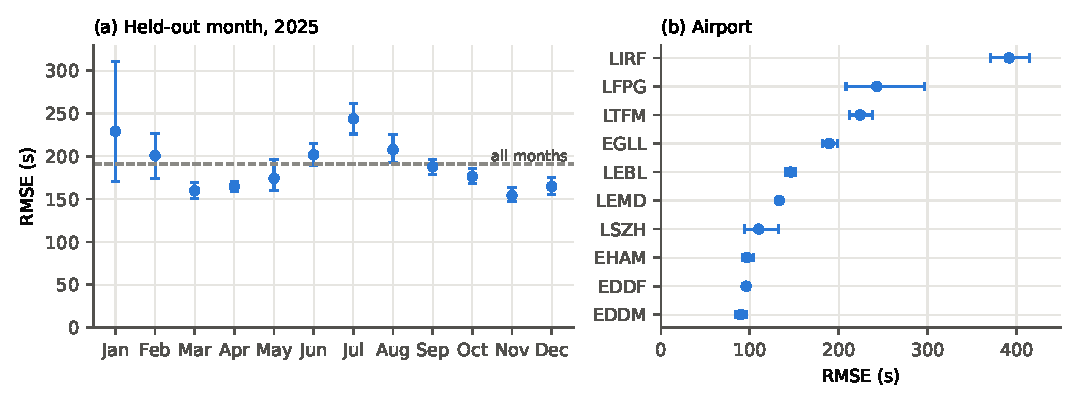
\includegraphics[width=\textwidth]{figures/validation_rmse.pdf}
  \caption{Month-held RMSE on 2025 departures, rollovers excluded, with 95\% day-block bootstrap intervals. (a) By held-out month; the dashed line is the all-month value of 191.1~s. (b) By airport.}
  \label{fig:validation}
\end{figure}

\subsection{Member accuracy and blend weights}

Table~\ref{tb:members} lists the month-held RMSE of each member in each lane, and the blend weights. The class-structured combiner is the best single model on matched departures in both delay bands, and it carries 98\% and 82\% of the blend weight there in the ten months with the full member list. On unmatched departures outside LIRF the transformer with stage-1 tokens is best (585.8 s); at LIRF the combiner trained only on unmatched departures is best (2,488.6 s). The two-stage XGBoost mixture is the weakest member at LIRF (4,208.7 s), and it and the per-airport CatBoost mixture are the weakest outside LIRF (659.2 s and 673.9 s); on these rows the distributional members and the combiner gain most. Overall, the blend is not measurably better than the combiner alone: 191.09 s against 191.12 s, a difference of $-0.02$ s (interval $-0.68$ to $+0.65$ s from 1,000 airport-day replicates without stratification). The blend therefore adds little to the combiner on the 2025 read.

\begin{table}[htbp!]
  \centering
  \small
  \caption{Month-held RMSE (s) of the members by lane, rollovers excluded, and blend weights for the full member list (in parentheses; weights below 0.01 omitted). n/a: member not in the full list for that lane. Member RMSEs are before window projection; the blend row is after it.}
  \label{tb:members}
  \begin{tabular}{lrrrr}
  \toprule
  \textbf{Member} & \textbf{FP, $C<1$ h} & \textbf{FP, $C \geq 1$ h} & \textbf{No FP, other} & \textbf{No FP, LIRF} \\
  \midrule
  Class-structured combiner & 149.2 (0.98) & 310.3 (0.82) & 592.3 (0.18) & 2,545.9 (0.19) \\
  Combiner, unmatched rows only & n/a & n/a & 590.9 & 2,488.6 (0.75) \\
  Four-class stamp model & 152.2 & 328.1 & n/a & n/a \\
  Transformer, base & 152.7 (0.01) & 321.3 (0.05) & n/a & n/a \\
  Transformer, stage-1 tokens & 154.2 & n/a & 585.8 (0.56) & 2,786.0 (0.06) \\
  Transformer, disruption tokens & 155.6 & 332.3 (0.05) & n/a & n/a \\
  Transformer, EOBT-free & n/a & 329.9 (0.04) & 594.1 (0.17) & n/a \\
  Transformer, unmatched rows upweighted & n/a & 327.8 & 591.4 (0.09) & n/a \\
  CatBoost mixture & 154.9 & 330.6 (0.04) & n/a & n/a \\
  CatBoost mixture per airport & 154.7 (0.01) & 332.4 & 673.9 & n/a \\
  Two-stage XGBoost, mixture & 157.6 & 349.8 & 659.2 & 4,208.7 \\
  \midrule
  Blend & 149.4 & 310.6 & 588.5 & 2,538.1 \\
  \bottomrule
  \end{tabular}
\end{table}

\subsection{Ablations and sensitivity}

\textit{Feature and member breadth.} Rebuilding the whole estimator on a reduced matrix of 75 columns with nine members raised the rollover-excluded RMSE from 191.1 s to 206.8 s (+15.7 s). The loss was largest where the label is hardest: +9.3 s on matched departures with $C<1$~h, +21.3 s with $C \geq 1$~h, +27 s on unmatched departures outside LIRF and +580 s on unmatched departures at LIRF.

\textit{Seeds.} Averaging the combiner over 17 seeds instead of one improved its RMSE by about 1.6 s. For the EOBT-free transformer on departures without a flight plan, the seed curve flattened after about ten seeds, and larger transformers (width 192, six layers) on these rows were worse than more seeds of the small model.

\textit{Feeder lateness.} Evaluated month-held on an earlier blend, offsets of the same form changed the overall RMSE by $-0.006$ s (interval $-0.010$ to $-0.002$ s) and improved 8 of 12 months. Their trigger is computable without labels.

\textit{Negative results.} Several ideas did not pass the decision rules: a retrieval-augmented tabular model in the style of TabR \cite{gorishniy2024tabr} (weak on its own, kept only as an auxiliary expert of the combiner); a queueing fixed-point model of the surface; per-cell blend refits beyond the four lanes, which showed a winner's curse across a scan of 51 cells; further stacking beyond the combiner on matched departures, where backward pruning showed that the combiner plus the simplex blend came within 0.3 s of a 51-member stack; transformers trained with long-delay rows upweighted, which were worse on that lane; day-level weather and de-icing offsets, for which the mechanism is real but month-to-month transfer failed (0 of 5 winter months improved); global offsets by delay band; and seasonal weighting of training months.

\subsection{Input drift and a label-free correction}
\label{sec:drift}

Applying the estimator to 2026 inputs exposed one large change in a single input. Figure~\ref{fig:drift} compares, for each airport and for January, February, June and July 2026, the mean of EOBT minus LOBT on matched departures with the same month of 2025. In 38 of the 40 airport-months the change lies between $-89$ s and $+50$ s. At LFPG in June and July 2026 it is $+240$ s and $+288$ s: the filed EOBT now sits about four to five minutes later relative to the LOBT. No 2025 month at LFPG resembles this, so the distribution of every feature anchored on the EOBT is shifted away from its 2025 distribution there.

\begin{figure}[htbp!]
  \centering
  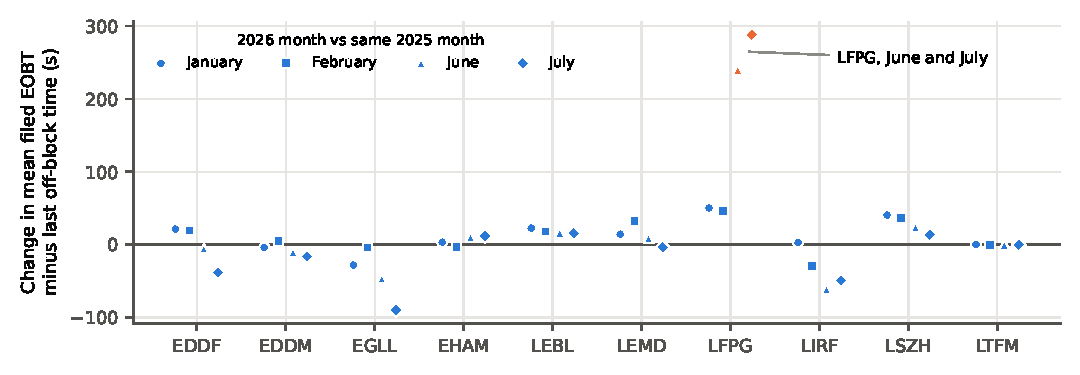
\includegraphics[width=\textwidth]{figures/eobt_drift.pdf}
  \caption{Change in the mean of filed EOBT minus LOBT, matched departures, between each 2026 month and the same month of 2025. Only LFPG in June and July (orange) moves by more than 90~s.}
  \label{fig:drift}
\end{figure}

Because the EOBT-free transformer does not see the drifted input, the mean difference between it and the transformer with stage-1 tokens on the affected cell estimates the bias the drift induces in EOBT-anchored members. The two models also differ in that the latter receives the stage-1 outputs, which are themselves anchored on the EOBT. Over LFPG departures with a flight plan and $C<1$~h, this difference was $+17.2$ s in July and $+16.0$ s in June (each from the pair of transformers that produced the estimate for that month, clamped to $\pm 60$ s), and it was added to those rows. The correction cannot be validated on 2025, which contains no such drift; it rests on the assumption that the EOBT-free model is unaffected and that the base model's bias equals the gap between the two. The same comparison of an ablated and a full model can be computed for any input suspected of drift, without labels; it complements label-free shift detection by two-sample tests \cite{rabanser2019failing}.

Two further changes in the 2026 inputs are relevant for future work: the share of LIRF departures with an ADS-B ground track fell from 0.956 in July 2025 to 0.002 in July 2026, and the share of departures without a flight plan at EHAM rose from 1.6\% in 2025 to 5.0\% in January 2026. Members trained with ADS-B features see an input state at LIRF that 2025 barely contains, The stack's routing of rows without a ground track to ADS-B-free twins (Section~\ref{sec:stack}) addresses this input state.


% =====================================================================================
\section{Discussion}
\label{sec:discussion}

\subsection{Modelling recording artefacts in the label}

The recorded off-block stamp is part of what has to be modelled. The flight-plan matching window gives a provable interval for 98.9\% of departures and makes the absence of a flight plan informative. Schedule-coincident stamps create a point mass whose value is known in advance, and at LIRF a probable recording practice makes this point mass almost a fifth of the airport's departures. Under squared error the target is the conditional mean of the recorded label \cite{gneiting2011making}, so these structures belong in the model. Trimming or cleaning them, as taxi-time studies commonly do \cite{wang2021aircraft,swatowska2025generalisable}, removes information that the error measure rewards. The label-noise literature describes such errors as noise not at random \cite{frenay2014classification}, and the econometric literature notes that misclassification-type errors in a response, unlike classical errors, bias what is learnt \cite{hausman2001mismeasured}. The class-structured combiner, which predicts class probabilities and class values and gates between experts only within the normal class, is the best single model on matched departures and carries most of the blend weight. A reduced build without the broader features and members lost 15.7 s, with the largest losses on long delays and on departures without a flight plan.

Operational uses, such as the taxi-out time that enters a target take-off time \cite{eurocontrol2017airport} or the fuel burnt on the ground \cite{khadilkar2012estimation}, need the physical duration. A recording-aware model provides an estimate of it through the normal-class component $\hat{y}_{\mathrm{normal}}$, which the mixture separates from the artefacts. The analysis of Section~\ref{sec:classes} also gives data owners a simple diagnostic: comparing the share of stamps that coincide with the schedule against the shares one minute either side separates minute-resolution recording from schedule defaults.

\subsection{Uncertainty and influential records in validation}

Two aspects of the validation affected decisions. First, intervals: the seed spread understated the day-block bootstrap uncertainty by one to two orders of magnitude, and a point-estimate decision rule accepted about a third of null changes. This agrees with evidence that data sampling contributes more to benchmark variance than initialisation does \cite{bouthillier2021accounting}. Second, influence: one record of 16.2 h holds 4.3\% of the squared error of two million departures and about 40\% of January's. Any comparison between models on such data must report results with and without these records, as we do for rollovers, and should report per-month and per-airport breakdowns rather than a single pooled number.

The literature on taxi-out prediction rarely reports intervals or validates on held-out periods (Section~\ref{sec:related}). Our month-held protocol is more demanding than a random split, and the RMSE values in Table~\ref{tb:results} are not comparable with values from random splits, from tactical prediction horizons, or from different label definitions.

\subsection{Training--serving skew in stacked estimators}

The estimator has three levels of stacking, and month-held validation measures each level only on consistent inputs. When we produced predictions from one-off retrains for months that the original runs had not covered, two stacked components behaved differently from their validated versions. We detected this without labels, from shifts in their mean predictions relative to sibling members, and excluded them for those months. A stacker's inputs at prediction time must come from the same procedure that generated its training inputs. This is the stacking version of training-serving skew \cite{breck2017ml,sculley2015hidden}, and month-held validation is blind to it by construction. A practical safeguard is to generate all folds of every member in a single run and to compare each member's prediction distribution on new inputs with that of its siblings.

\subsection{Label-free estimates of input drift}

Inputs can change in ways that 2025 data cannot anticipate: a change in how EOBTs are filed at LFPG, the near-disappearance of ADS-B ground coverage at LIRF in July 2026, and a higher share of departures without a flight plan at EHAM in January 2026. A model with an ablated input (here, without EOBT-anchored features) provides a label-free estimate of the bias that a drifted input induces in the full model. The estimate rests on two assumptions: that the ablated model is unaffected by the drift, and that the two models would otherwise agree on average. The second can be checked on 2025 data; the first, like the size of the correction, cannot be checked until labels for the drifted period are available. Here the two models also differ in their stage-1 inputs.

\subsection{Limitations}

The estimator is post-operational: it uses the take-off time, the arrivals' in-block times and flight-plan fields that are known only after the fact, so its accuracy says nothing about tactical prediction before off-block. All quantitative results are month-held estimates on 2025; they transfer to 2026 only insofar as 2026 resembles 2025, which Section~\ref{sec:drift} shows is not entirely true. The matching window, the recording classes and the arrival-twin inference are properties of this dataset and its matching procedure; other data sources will have different structures, although the approach of identifying and modelling them carries over. The 3,606 s tolerance is inferred from the data, not documented. The comparative evidence we cite for tabular models comes mostly from benchmarks of moderate size with random splits \cite{grinsztajn2022why,mcelfresh2023when,erickson2025tabarena}, which may not transfer to a temporally shifting dataset of two million rows. Several members train on GPUs and reproduce only up to hardware nondeterminism \cite{pham2020problems}. Finally, the decision rules were fixed in advance but not formally registered.


% =====================================================================================
\section{Conclusion}
\label{sec:conclusion}

We built an estimator of recorded taxi-out time for 2,085,047 departures at ten European airports and organised it around the structure of the label. An inferred flight-plan matching window gives most departures a provable label interval and makes a missing flight plan informative. Off-block stamps that coincide with the schedule form a point mass, and at one airport a recording practice makes it large. Gradient-boosted trees, a distributional transformer with a masked histogram head, and a class-structured combiner whose experts include an earlier stack of tabular, sequence and set models each model the label as a mixture of recording classes. A per-lane non-negative blend and label-free projections complete the estimator. Under month-held, nested validation with day-block bootstrap intervals, the blend reaches an RMSE of 191.1 s (183.5 to 201.7 s) with rollovers excluded and 227.4 s on all records, with most of the error in departures without a flight plan and in long delays. Three practical points follow for future work on recorded operational durations: model the recorded label rather than an idealised one, validate on held-out periods with calibrated intervals, and keep the inputs of stacked models consistent between training and prediction.


% =====================================================================================
\appendix

\section{Settings of the main members}
\label{app:settings}

\begin{table}[htbp!]
  \centering
  \small
  \caption{Main settings of the members trained on the compact feature matrix. All members are trained 13 times (12 held-out months and the full year). Day-rollover rows are excluded from training.}
  \label{tb:settings}
  \begin{tabular}{p{0.26\textwidth}p{0.68\textwidth}}
  \toprule
  \textbf{Component} & \textbf{Settings} \\
  \midrule
  Stage-1 XGBoost & offset model: squared error, 1,500 rounds, depth 10, learning rate 0.05, minimum child weight 200, $L_2$ penalty 5; quantile models (10th, 50th, 90th percentile): 800 rounds, depth 8; class models (schedule coincidence; label $>$ 1 h): logistic, 800 rounds, depth 8, minimum child weight 50; histogram method on GPU with native categorical handling; inner month-held folds over the 11 training months \\
  Stage-2 XGBoost & 2,500 rounds, depth 10, learning rate 0.03, minimum child weight 1,000, $L_2$ penalty 10 \\
  CatBoost mixture & classifier 3,000 iterations, depth 8; depth-wise regressor 8,000 iterations, depth 10 \\
  CatBoost mixture per airport & per airport: classifier 2,000 iterations, depth 6; matched-row label regressor 5,000 iterations, depth 10; unmatched-row regressor 1,500 iterations, depth 6 (airport median when 200 or fewer training rows) \\
  Four-class stamp model & multiclass CatBoost, 4,000 iterations, depth 8; normal class: bounded-offset regressor (matched rows; 8,000 iterations, depth 10) or label regressor (unmatched rows; 3,000 iterations, depth 8); near-schedule and long classes: 2,000 iterations, depth 6 \\
  Distributional transformer & 3 pre-norm layers, width 64, 4 heads, feed-forward width 128, dropout 0.1, GELU; head: linear, GELU, linear to $K+1$ logits; bins 20 s to 3,600 s, 120 s to 14,400 s; HL-Gauss $\sigma$ = 0.75 bin widths; loss: cross-entropy + $10\cdot$MSE$/10^6$; AdamW, learning rate $5\times10^{-4}$, weight decay $10^{-5}$, one-cycle schedule, batch 1,024, 6 epochs, bfloat16; 3 to 18 seeds per variant \\
  Class-structured combiner & airport embedding of width 8 plus context; two hidden layers of 256 units, SiLU, dropout 0.1; zero-initialised gate and adjustment heads; loss MSE$/10^4$ + 0.1 cross-entropy; AdamW, learning rate $10^{-3}$, weight decay $10^{-4}$, batch 4,096, 10 epochs; 17 seeds (all departures) and 45 seeds (unmatched departures) \\
  Blend & four lanes; non-negative least squares with ridge row $\lambda = 10^3\sqrt{n}$ toward equal weights; weights normalised to sum to one \\
  \bottomrule
  \end{tabular}
\end{table}


\section*{Acknowledgement}
This work was carried out as part of the PRC Data Challenge 2026 organised by the EUROCONTROL Performance Review Commission with the support of the OpenSky Network \cite{performancereviewcommission2026prc}. We thank the organisers for preparing and releasing the movement and flight data and for their support during the challenge. ADS-B ground tracks contain data from ADSB.lol, made available under the Open Database License (ODbL) 1.0. Map data \textcopyright{} OpenStreetMap contributors. Weather data by Open-Meteo.com.

\section*{Author contributions}
All authors contributed equally to this work. Each author contributed to Conceptualization, Data Curation, Formal Analysis, Investigation, Methodology, Project Administration, Resources, Software, Validation, Visualization, Writing (Original Draft) and Writing (Review and Editing).

\section*{Funding statement}
This research received no funding.

\section*{Open data statement}
The 2025 movement and flight data were provided by the EUROCONTROL Performance Review Commission (see Acknowledgement). All external data used by the estimator are openly available: ADS-B traces from the ADSB.lol global history archive (ODbL 1.0) \cite{adsblol2026historical}, runway data from OurAirports (public domain) \cite{ourairports2026open}, taxiway geometry from OpenStreetMap (ODbL 1.0) \cite{haklay2008openstreetmap}, stand data from the X-Plane Scenery Gateway \cite{xplane2026scenery}, METAR reports from the Iowa Environmental Mesonet \cite{iem2026download}, hourly weather from Open-Meteo (CC BY 4.0) \cite{zippenfenig2023openmeteo} and daily airport arrival air traffic flow management delay from EUROCONTROL \cite{eurocontrol2026airport}. The repository documents the source of each external dataset; derived ADS-B tables are rebuilt by script and not redistributed.

\section*{Reproducibility statement}
All code is available at \url{https://github.com/JuanesLamilla/PRC-2026-humble-rocket} under the GNU General Public License v3.0 or later. The repository contains the data preparation and feature code, the member scripts with a reconstructed record of the training runs (tags, flags and seeds; the full command lines of historical runs were not retained), the blend and post-processing code, and the scripts for the figures and tables of this paper (in the \texttt{manuscript} folder). Members were trained on NVIDIA H200 and L40S GPUs; GPU training is seeded but not bit-deterministic, so retrained members reproduce our predictions up to hardware nondeterminism. Given the member outputs, the blend and post-processing are deterministic and reproduce our estimates byte for byte.

\printbibliography

\end{document}
